%!TEX TS-program = xelatex
\documentclass[a4paper,14pt]{article}
\usepackage[utf8]{inputenc}
\usepackage[T1]{fontenc}

%%% Работа с русским языком
\usepackage[english,russian]{babel}   %% загружает пакет многоязыковой вёрстки
\usepackage{fontspec}      %% подготавливает загрузку шрифтов Open Type, True Type и др.
\defaultfontfeatures{Ligatures={TeX},Renderer=Basic}  %% свойства шрифтов по умолчанию
\setmainfont[Ligatures={TeX,Historic}]{Times New Roman} %% задаёт основной шрифт документа
\setsansfont{Comic Sans MS}                    %% задаёт шрифт без засечек
\setmonofont{Courier New}
\usepackage{indentfirst}
\frenchspacing

\renewcommand{\epsilon}{\ensuremath{\varepsilon}}
\renewcommand{\phi}{\ensuremath{\varphi}}
\renewcommand{\kappa}{\ensuremath{\varkappa}}
\renewcommand{\le}{\ensuremath{\leqslant}}
\renewcommand{\leq}{\ensuremath{\leqslant}}
\renewcommand{\ge}{\ensuremath{\geqslant}}
\renewcommand{\geq}{\ensuremath{\geqslant}}
\renewcommand{\emptyset}{\varnothing}

%%% Дополнительная работа с математикой
\usepackage{amsmath,amsfonts,amssymb,amsthm,mathtools} % AMS
\usepackage{icomma} % "Умная" запятая: $0,2$ --- число, $0, 2$ --- перечисление

%% Номера формул
%\mathtoolsset{showonlyrefs=true} % Показывать номера только у тех формул, на которые есть \eqref{} в тексте.
%\usepackage{leqno} % Нумерация формул слева	

%% Перенос знаков в формулах (по Львовскому)
\newcommand*{\hm}[1]{#1\nobreak\discretionary{}
{\hbox{$\mathsurround=0pt #1$}}{}}

%%% Работа с картинками
\usepackage{graphicx}  % Для вставки рисунков
\graphicspath{{images/}}  % папки с картинками
\setlength\fboxsep{3pt} % Отступ рамки \fbox{} от рисунка
\setlength\fboxrule{1pt} % Толщина линий рамки \fbox{}
\usepackage{wrapfig} % Обтекание рисунков текстом

%%% Работа с таблицами
\usepackage{array,tabularx,tabulary,booktabs} % Дополнительная работа с таблицами
\usepackage{longtable}  % Длинные таблицы
\usepackage{multirow} % Слияние строк в таблице
\usepackage{float}% http://ctan.org/pkg/float

%%% Программирование
\usepackage{etoolbox} % логические операторы


%%% Страница
\usepackage{extsizes} % Возможность сделать 14-й шрифт
\usepackage{geometry} % Простой способ задавать поля
\geometry{top=20mm}
\geometry{bottom=20mm}
\geometry{left=20mm}
\geometry{right=10mm}
%
%\usepackage{fancyhdr} % Колонтитулы
% 	\pagestyle{fancy}
%\renewcommand{\headrulewidth}{0pt}  % Толщина линейки, отчеркивающей верхний колонтитул
% 	\lfoot{Нижний левый}
% 	\rfoot{Нижний правый}
% 	\rhead{Верхний правый}
% 	\chead{Верхний в центре}
% 	\lhead{Верхний левый}
%	\cfoot{Нижний в центре} % По умолчанию здесь номер страницы

\usepackage{setspace} % Интерлиньяж
\onehalfspacing % Интерлиньяж 1.5
%\doublespacing % Интерлиньяж 2
%\singlespacing % Интерлиньяж 1

\usepackage{lastpage} % Узнать, сколько всего страниц в документе.

\usepackage{soul} % Модификаторы начертания

\usepackage[hyphens]{url}
\usepackage{hyperref}
\usepackage[usenames,dvipsnames,svgnames,table,rgb]{xcolor}
\hypersetup{                % Гиперссылки
    unicode=true,           % русские буквы в раздела PDF
    pdftitle={Детекция объектов по нескольким примерам без дообучения},   % Заголовок
    pdfauthor={Самоделкина М.В., Подчезерцев А.Е.},      % Автор
    pdfsubject={Детекция объектов по нескольким примерам без дообучения},      % Тема
    pdfcreator={Самоделкина М.В., Подчезерцев А.Е.}, % Создатель
    pdfproducer={Самоделкина М.В., Подчезерцев А.Е.}, % Производитель
%    pdfkeywords={keyword1} {key2} {key3}, % Ключевые слова
    colorlinks=true,        % false: ссылки в рамках; true: цветные ссылки
    linkcolor=black,          % внутренние ссылки
    citecolor=black,        % на библиографию
    filecolor=magenta,      % на файлы
    urlcolor=black           % на URL
}
\makeatletter
\def\@biblabel#1{#1. }
\makeatother
\usepackage{cite} % Работа с библиографией
%\usepackage[superscript]{cite} % Ссылки в верхних индексах
%\usepackage[nocompress]{cite} % 
\usepackage{csquotes} % Еще инструменты для ссылок

\usepackage{multicol} % Несколько колонок

\usepackage{tikz} % Работа с графикой
\usepackage{pgfplots}
\usepackage{pgfplotstable}

\usepackage{ dsfont }

\newcommand{\imref}[1]{рис.~\ref{#1}}

\usepackage{multirow}
\usepackage{spreadtab}
\newcolumntype{K}[1]{@{}>{\centering\arraybackslash}p{#1cm}@{}}


\usepackage{xparse}
\usepackage{fancyvrb}

\RecustomVerbatimCommand{\VerbatimInput}{VerbatimInput}
{
    fontsize=\footnotesize
}

\newcolumntype{?}[1]{!{\vrule width #1}}

\usepackage{tocloft}
\renewcommand{\cftsecleader}{\cftdotfill{\cftdotsep}}

\usepackage{pdfpages}

\usepackage{rotating}

\usepackage{pdflscape}

\usepackage{ragged2e}
\usepackage{microtype}

\usepackage{subcaption}

% Выравнивание по ширине без переносов слов
\justifying
\sloppy
\tolerance=500
\hyphenpenalty=10000
\emergencystretch=3em

% Подогнать таблицу под ширину страницы
\usepackage{adjustbox}

\usepackage{titlesec}

% ГОСТ заголовки таблицы
\usepackage[font=small]{caption}

\captionsetup[figure]{justification=centering,labelsep=period} % Картинки по центру, с точкой после рис

\DeclareCaptionLabelFormat{rightline}{\rightline{\bothIfFirst{#1}{ }#2}}
%\captionsetup[table]{justification=centering,labelformat=rightline,labelsep=newline}
\captionsetup[table]{justification=raggedleft,labelformat=rightline,labelsep=newline}

\newcommand{\tablecaption}[1]{\addtocounter{table}{1}\small \begin{flushright}
                                                                \tablename \ \thetable
\end{flushright}%
    \begin{center}
        #1
    \end{center}}

\usepackage{enumerate}

%сноска с новым номером на кждоый странице
\usepackage[perpage]{footmisc}
\usepackage[fixlanguage]{babelbib}
\usepackage{lastpage}
\begin{document}

    \begin{titlepage}
    \begin{center}
        ПРАВИТЕЛЬСТВО РОССИЙСКОЙ ФЕДЕРАЦИИ \\
        ФЕДЕРАЛЬНОЕ ГОСУДАРСТВЕННОЕ АВТОНОМНОЕ \\
        ОБРАЗОВАТЕЛЬНОЕ УЧРЕЖДЕНИЕ ВЫСШЕГО ОБРАЗОВАНИЯ\\
        «НАЦИОНАЛЬНЫЙ ИССЛЕДОВАТЕЛЬСКИЙ УНИВЕРСИТЕТ\\
        «ВЫСШАЯ ШКОЛА ЭКОНОМИКИ»
    \end{center}

    \begin{center}
        \textbf{Факультет компьютерных наук}

        \textbf{Образовательная программа <<Финансовые технологии и анализ данных>>}

%        \vspace{2ex}

    \end{center}
    \vspace{1ex}

    \begin{center}
        \textbf{Курсовая работа \\
            <<Детекция объектов по нескольким примерам без дообучения>>
        }
    \end{center}

    \vspace{2ex}
    \vfill

    \vspace{2ex}

    \begin{flushright}
        \textbf{Выполнили:}

        \vspace{2ex}

        Студенты группы мФТиАД21

        \vspace{2ex}

        Самоделкина Мария Владимировна

        Подчезерцев Алексей Евгеньевич

        \vspace{2ex}
        \textbf{Руководитель:}

        Приглашенный преподаватель

        Озерин Алексей Юрьевич

    \end{flushright}

    \vspace{5ex}
    \begin{center}
        Москва \the\year \, г.
    \end{center}

\end{titlepage}
\addtocounter{page}{1}

    \section*{\normalsize \hfill Аннотация \hfill}

    Что попробовали, что получили

    \sloppy
    \newpage

    \section*{\normalsize \hfill Abstract \hfill}

    ...

    \newpage

    \tableofcontents
    \pagebreak

    \section*{Введение}
    \addcontentsline{toc}{section}{\protect\numberline{}Введение}

	Большое количество существующих алгоритмов детекции объектов обучаются на заранее заданные классы изображений. 
	Для обучения таких моделей требуется объемная обучающая выборка с объектами каждого класса. 
	Однако сбор выборки для объектов редких категорий может быть затруднителен.
	В таком случае применение подхода с дообучением по нескольким примерам позволит не ограничиваться конкретными классами и решить проблему сбора данных для редких категорий.
	
	Кроме того, может возникнуть необходимость уточнить и сузить категорию, на которую уже обучена модель, или найти изображение по его описанию.
	Для решения данной задачи существуют подходы, позволяющие производить поиск объектов по произвольному текстовому запросу без дообучения.
	Однако требуется дополнительное исследование подходов детекции объектов по произвольному текстовому запросу, поскольку существующие решения имеют потенциал для улучшения эффективности или имеют ограничения по использованию.
	
	Более того, помимо детекции объекта на изображении иногда требуется находить его ключевые точки.
	Для этой задачи также не всегда имеется возможность собрать большую обучающую выборку.
	В связи с этим в работе исследуется возможность обучения модели нахождения ключевых точек по нескольким примерам.

    \newpage


    \section{Теоретическая часть}

    \subsection{Основные понятия}

    Задача детекции объектов (object detection) на изображении включает в себя несколько подзадач:
    \begin{enumerate}
        [1)]
        \itemsep0em
        \item определение прямоугольной области, ограничивающей объект (bounding box, bbox);
        \item классификация выделенной области;
    \end{enumerate}
    В результате работы модели, решающей задачу поиска объектов, получаются области или регионы изображения (object proposals) в которых может находиться объект, а также определена вероятность принадлежности этого объекта к определенному классу.

    Дополнительно могут решаться задачи нахождения ключевых точек объекта и сегментации - отделения объекта от фона, нахождение маски объекта.

    Наиболее популярные датасеты для обучения модели детекции объектов: MS~COCO~\cite{COCO}, LVIS~\cite{LVIS}, Objects365~\cite{Objects365}.
    Датасет LVIS содержит 164 тысячи изображений для решения задачи сегментации. Разработчиками предоставлена высококачественная разметка для более 1200 различных категорий.
    % TODO как оценивают качество в lvis по категориям

    Эмбеддинг (embedding) -- скрытое векторное представление объекта (текстовых, графические, табличных и аудио данных) фиксированной размерности.

    Карта признаков (feature map) -- векторное представление изображения нефиксированной размерности, где элемент карты содержит информацию о некоторой области изображения.

    NMS (non-maximum suppression)~\cite{neubeck2006efficient} -- алгоритм выделения регионов изображения с максимумом уверенности в классификации.
    В данном алгоритме объединяются регионы, отношение площади пересечения к объединению (IoU, Intersection over Union) которых больше заданного порога.
    Алгоритм позволяет получить из большого числа похожих или маловероятных регионов изображений один или несколько малопересекающихся регионов.

    \subsection{Модели для решения задачи детекции объектов}

    Mask R-CNN (Regions With CNNs)~\cite{MaskRCNN} -- двухэтапная нейронная сеть, позволяющая решать задачи детекции объектов и сегментации. В основе сети лежит сверточная нейронная сеть FCN (Fully Convolutional Network), состоящая только из сверточных (convolution) слоев и слоев подвыборки (pooling). Первый модуль RPN (Region Proposal Network) позволяет выделить регионы изображения по карте признаков сверточной нейронной сети. Вторым этапом происходит предсказание bounding box, класса и маски объекта для каждого региона.

    YOLO (You Only Look Once)~\cite{redmon2016you} -- семейство архитектур моделей, позволяющее ускорить решение задачи детекции объектов и получать результаты в режиме реального времени.
    Это одноэтапная нейронная сеть, не использующая модуль для выделения регионов изображения.
    В модели сначала получают карты признаков для изображения с помощью сверточных слоев (backbone часть), далее для каждого элемента карты решаются задачи определения класса объекта и его размеров, центр которого находится в данном элементе карты (head часть).
    В модели используется 3 карты признаков различных размеров: каждая последующая получается применением набора сверток к предыдущей.
    Такой подход используется для нахождения объектов разных размеров -- маленьких, средних и больших.
    Модели YOLO обучены на датасете COCO, содержащем 80 категорий.

    CLIP (Contrastive Language–Image Pre-training)~\cite{CLIP} -- модель, позволяющая переводить текстовые описания и изображения в единое векторное пространство.
    CLIP предоставляет возможность решать задачу детекции объектов без дообучения для произвольных классов.
    В основе модели лежат Text Encoder и Image Encoder для преобразования текста и изображения в векторные представления, косинусное расстояние между которыми максимизируется для релевантных пар текста и изображения и минимизируется для нерелевантных.

    \subsection{Приблизительный поиск ближайших соседей}

    Для поиска похожих эмбеддингов среди набора заранее заданных эмбеддингов используют методы приблизительного поиска ближайших соседей.
    Такие алгоритмы позволяют ускорить поиск, по сравнению с полным перебором всех объектов, однако требуют дополнительных затрат на построение индекса,
    могут возвращать не самых ближайших соседей, а только приближенных к ним.
    В основе таких методов лежат алгоритмы 
    \begin{enumerate}
    	[1)]
    	\itemsep0em
    	\item вероятностного хеширования~\cite{tao2010efficient}, которые проецируют похожие объекты в одинаковые корзины (buckets), после этого осуществляется поиск ближайших соседей среди объектов корзины;
    	\item деревев поиска~\cite{liu2006new}, которые разделяют все пространство на небольшие подпространства и проводят поиск среди части объектов в подпространстве;
    	\item построения графов~\cite{malkov2018efficient}, где вершинами являются исходные эмбеддинги, а
    	ребра~--~связи между близкими вершинами, поиск кандидатов осуществляется жадным блужданием по графу.
    \end{enumerate}
    Различные комбинации и оптимизации алгоритмов построения индекса и поиска позволяют дополнительно сократить время поиска объекта или повысить точность результатов~\cite{annoy,avq_2020}.

    \subsection{Выводы к главе \thesection}
    \begin{enumerate}
        \itemsep0em
        \item Выделены основные понятия и рассмотрены модели, необходимые для решения задачи детекции объектов.
        \item Изучен алгоритм поиска ближайших соседей, который используется в работе для поиска похожих эмбеддингов.
    \end{enumerate}

    \newpage


    \section{Обзор литературы}

    \subsection{Детекция объектов по произвольному текстовому запросу}

    В статье~\cite{ViLD} предложен метод ViLD - Vision and Language knowledge Distillation, позволяющий находить объекты с произвольным текстовым описанием.
    На этапе обучения рассчитываются текстовые эмбеддинги описаний категорий и эмбеддинги регионов изображения с использованием предобученной модели (модель-учитель).
    Обучается модель детекции объектов Mask R-CNN (модель-ученик), которая дополнительно максимизирует расстояние между эмбеддингом региона предобученной модели-учителя и эмбеддингами региона модели-ученика.
    Таким образом, происходит извлечение знаний (дистилляция) из модели-учителя.
    Во время применения модели-ученика предобученная модель-учитель используется только для получения текстовых эмбеддингов, а эмбеддинги для регионов получается из модели-ученика.
    Итоговые регионы получаются в результате ранжирования оценок, полученных как скалярное произведение текстового эмбеддинга модели-учителя и эмбеддинга региона модели-ученика.

    В качестве модели-учителя в статье используется модель CLIP.
    Модель обучена на датасете LVIS.
    В работе отмечается, что модель может применяться и к другим датасетам (COCO, Objects365) без дообучения.

    Преимуществом описанного подхода является использование одной модели как для выделения регионов, так и для получения их эмбеддингов, что ускоряет время применения, однако точность при таком подходе понижается.

    Полученную модель предлагается использовать следующим образом: для изображения подавать набор текстовых описаний и отбирать заданное количество регионов с минимальным скалярным произведением.

    К недостаткам предлагаемого подхода можно отнести поиск текстовых описаний только на одном изображении, то есть при отсутствии объектов, релевантных набору текстовых описаний, алгоритм выведет требуемое количество регионов (для нерелевантных текстовых описаний скалярное произведение также может быть высокое).
    
    В работе~\cite{detpro} представлен метод DetPro (Detection Prompt), улучшающий метод ViLD. 
    DetPro позволяет предсказывать наиболее подходящий контекст для поискового запроса к модели CLIP, в то время как в методе ViLD контекст подбирался вручную.
    Метод DetPro позволяет определять уровень контекста на изображении, например, полностью изображен объект или частично.
    Также представлена доработка, позволяющая минимизировать схожесть текстового эмбеддинга запроса и эмбеддинга фона изображения.
    Предлагаемый метод улучшает результаты статьи~\cite{ViLD}, поскольку текстовый контекст существенно влияет на результаты детекции.

    \subsection{Детекция объектов редких категорий по нескольким примерам}
    
    Предлагаемый в статье~\cite{FSODFeatureReweighting} подход позволяет находить объекты новых классов при дообучении по нескольким примерам.
    Модель, предлагаемая в подходе, состоит из двух частей: 
     \begin{enumerate}
    	[1)]
    	\itemsep0em
    	\item feature learner - модуль для получения признаков, хорошо описывающих как базовые, так и редкие классы. 
    	В работе в качестве feature learner используется одностадийный детектор YOLOv2;
    	\item reweighting module - простая сверточная модель, применяемая для детекции каждого класса. Модель учится извлекать релевантные для класса признаки feature learner модуля.
    \end{enumerate}
	В соответствии с данным подходом в статье предлагается специальная двухэтапная схема обучения: обучение на базовые классы и дообучение на базовые и редкие классы.

    В работе~\cite{wang2020few} авторы предлагают двушаговый алгоритм дообучения моделей для детекции на нескольких примерах.
    %Кроме того, используются метрики качества, оценивающие качество работы модели на популярных или на редких изображениях.
    На первом этапе обучается модель на объектах базовых классов, которые часто встречаются в выборке.
    На следующем этапе предлагается заморозить все веса сети, кроме последнего, и обучать модель на выборке, состоящей из частых и редких объектов в равных пропорциях.
    Авторы используют несколько датасетов -- COCO, LVIS и PASCAL VOC,
    и несколько архитектур моделей -- Faster R-CNN, VGG16, YOLOv2, для проверки своих гипотез.
    Предлагаемый в статье подход позволил повысить качество работы моделей на несколько пунктов, в зависимости от датасета и модели.
    
    % Подход не подходит, когда редкие категории заранее неизвестны

    \subsection{Инженерный подход к разметке изображений}

    В решении~\cite{AnnoMage} реализован подход для полу-автоматизированной разметки датасетов изображений.
    В предложенном приложении автоматически размечаются области, соответствующие выбранным классам датасета COCO, полученные с помощью загруженной модели.

    В отличие от решения ~\cite{AnnoMage} в курсовой работе предлагается подход с дообучением модели на новой разметке и применением модели для произвольных текстовых запросов.

    \subsection{Цель и задачи исследования}
    
    Целью данной работы является разработка подхода к детекции объектов произвольному текстовому запросу.
    
    Провести анализ существующих моделей детекции объектов и выбрать на основе метрик качества лучшую реализацию.
    
    Подобрать алгоритм поиска ближайших соседей, ускоряющий выдачу изображений.
    
    Разработать модуль, позволяющий улучшать разметку выдачи и дообучать модель детекции.
    
    Предлагаемый подход можно применять также для отбора наиболее релевантных изображений из пользовательского датасета.

    В работе решаются следующие задачи:
    \begin{enumerate}
        [1)]
        \itemsep0em
        \item анализ существующих решений задачи детекции объектов и алгоритмов поиска ближайших соседей;
        \item реализация предлагаемого подхода и выбор наиболее оптимальной модели для детекции объектов по произвольному текстовому запросу;
        \item демонстрация результатов работы предлагаемого подхода и улучшение результатов выдачи;
        \item исследование подхода для решения задачи регрессии ключевых точек с дообучением по нескольким примерам;
        \item анализ проведенных экспериментов и составление рекомендаций по использованию полученных результатов.
    \end{enumerate}

    \subsection{Выводы к главе \thesection}
    \begin{enumerate}
        \itemsep0em
        \item Рассмотрены подходы к детекции объектов по произвольному текстовому запросу, к детекции объектов редких категорий по нескольким примерам и инженерный подход к разметке изображений.
        \item Сформулированы цель и задачи исследования.
    \end{enumerate}

    \newpage


    \section{Практическая часть}

    \subsection{Описание данных}
    %TODO Более подробно про датасет LVIS, какие категории, сколько редких

    \subsection{Подход к детекции объектов по произвольному запросу}

    Целью данного подхода является выделение заданного количества наиболее релевантных изображений по произвольному текстовому описанию.
    Подход реализуется в несколько этапов:
    \begin{enumerate}
        [1)]
        \itemsep0em
        \item получение регионов для всего доступного множества изображений;
        \item вычисление векторного представления регионов и текстового запроса;
        \item поиск ближайших регионов к текстовому запросу.
    \end{enumerate}

    При проведении эксперимента для оценки качества предлагаемого подхода используются изображения датасета LVIS.

    В качестве модели для выделения регионов использовались модели YOLOv5 и ViLD.
    Исходная модель YOLOv5 была модифицирована таким образом, чтобы в результате применения модели получалось как можно больше регионов.
    Для этого уменьшался порог уверенности модели в классификации и для объединения похожих регионов использовался модифицированный алгоритм NMS.

    В измененном алгоритме NMS не учитывается предсказанный класс объекта	~--~это сделано для того, чтобы получать регионы для объектов, на которые модель не была обучена.
    Чтобы избавиться от дублированных регионов к ограничивающей области была применена кластеризация методом k-средних с заданным максимальным количеством кластеров, после чего к областям одного кластера применялся классический алгоритм NMS.
    На рис.~\ref{fig:nms} продемонстрирован результат работы модифицированного алгоритма NMS: результат кластеризации дублированных регионов представлен на рис.~\ref{fig:nms1}, кластера отмечены одним цветом; итоговый результат применения NMS к выделенным кластерам изображен на рис.~\ref{fig:nms2}~--~количество выделенных регионов существенно уменьшено.

    \begin{figure}[H]
        \centering
        \begin{subfigure}{.5\textwidth}
            \centering
            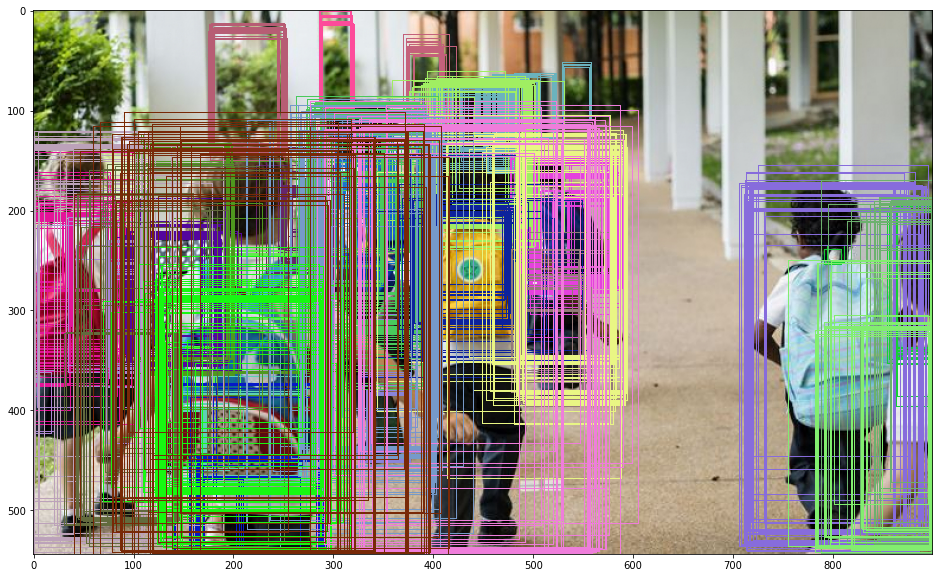
\includegraphics[width=\linewidth]{images/before_nms}
            \caption{Результат кластеризации регионов}
            \label{fig:nms1}
        \end{subfigure}%
        \begin{subfigure}{.5\textwidth}
            \centering
            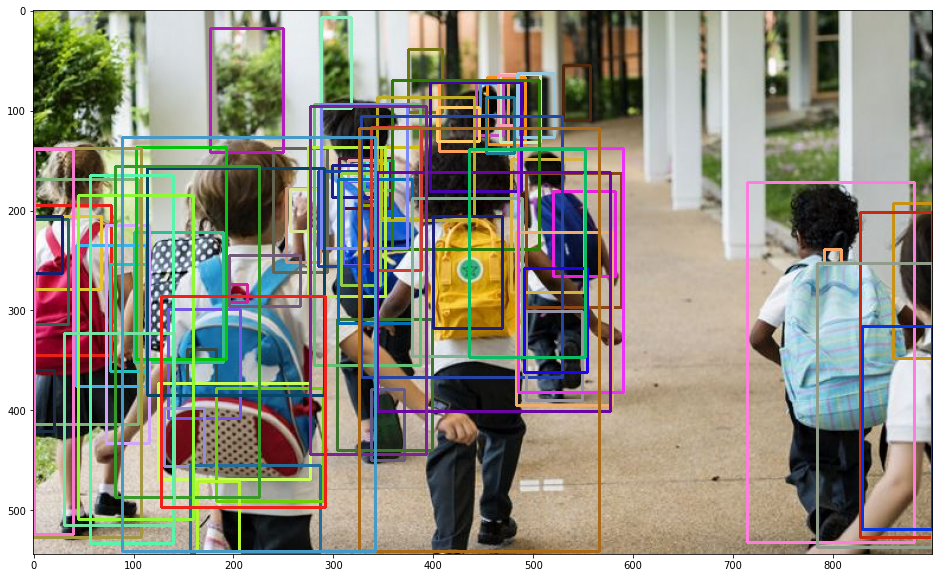
\includegraphics[width=\linewidth]{images/after_nms}
            \caption{Результат применения NMS к кластерам}
            \label{fig:nms2}
        \end{subfigure}
        \caption{Демонстрация работы модифицированного алгоритма NMS}
        \label{fig:nms}
    \end{figure}

    При проведении эксперимента количество кластеров для метода k-средних определялось по следующей формуле:
    $\max(\min(30, \left[\frac{m}{2}\right]), 1),$ где $m$~--~количество найденных на изображении регионов.
    Для проведения расчетов использовались также следующие гиперпараметры, представленные в таблице~\ref{tab:base_params}.

    \begin{center}
        \begin{table}[H]
            \centering
            \caption{Параметры алгоритма детекции объектов}
            \label{tab:base_params}
            \bgroup
            \def\arraystretch{1.5}
            \begin{tabular}{| l | l |}
                \hline
                Порог уверенности модели в классификации & 0,01 \\ \hline
                Пороговое значение IoU                   & 0,45 \\ \hline
                Максимальное количество регионов в NMS   & 10   \\
                \hline
            \end{tabular}
            \egroup
        \end{table}
    \end{center}

    Далее для каждого выделенного региона изображения применялась модель CLIP.
    Текстовый запрос также переводился в векторное пространство с помощью этой модели.
    Для тестирования подхода в качестве текстовых запросов использовались определения категорий датасета LVIS.

    С помощью приблизительного поиска ближайших соседей, а также полным перебором по максимизации косинусного расстояния для сравнения результатов осуществлялся поиск заданного количества ближайших векторов регионов к вектору текстового запроса (определению категории).

    Таким образом, для повышения точности среди выбранных изображений в предлагаемом подходе последовательно используются 2 модели: YOLOv5 или ViLD, CLIP.

    В качестве эксперимента также было проведено сравнение качества модели ViLD при использовании только результатов выделения регионов, а также с использованием эмбеддинга региона из модели ViLD.
    В последнем случае модель CLIP не применялась к найденным регионам.
    Результаты экспериментов описаны в п.~\ref{fsod_exp}.

    \subsection{Решение задачи регрессии ключевых точек}

    В курсовой работе исследован подход к решению задачи регрессии ключевых точек с дообучением по нескольким примерам.
    Задача решается в несколько этапов:
    \begin{enumerate}
        [1)]
        \itemsep0em
        \item получение карты признаков для входящего набора изображений с помощью предобученной модели;
        \item обучение нескольких моделей линейной регрессии для нахождения каждой ключевой точки.
    \end{enumerate}
    При проведении эксперимента в качестве предобученной модели использовалась YOLOv5.
    На рис.~\ref{fig:stage9_SPPF_features} представлена визуализация элементов (матриц) последнего слоя backbone части модели YOLOv5. На представленном рисунке матрица имеет размерность 20×15. Вектор получаемой карты признаков (количество матриц) имеет размерность 1280, один элемент матрицы соответствует 32 пикселям исходного изображения.
    \begin{figure}[H]
        \centering
        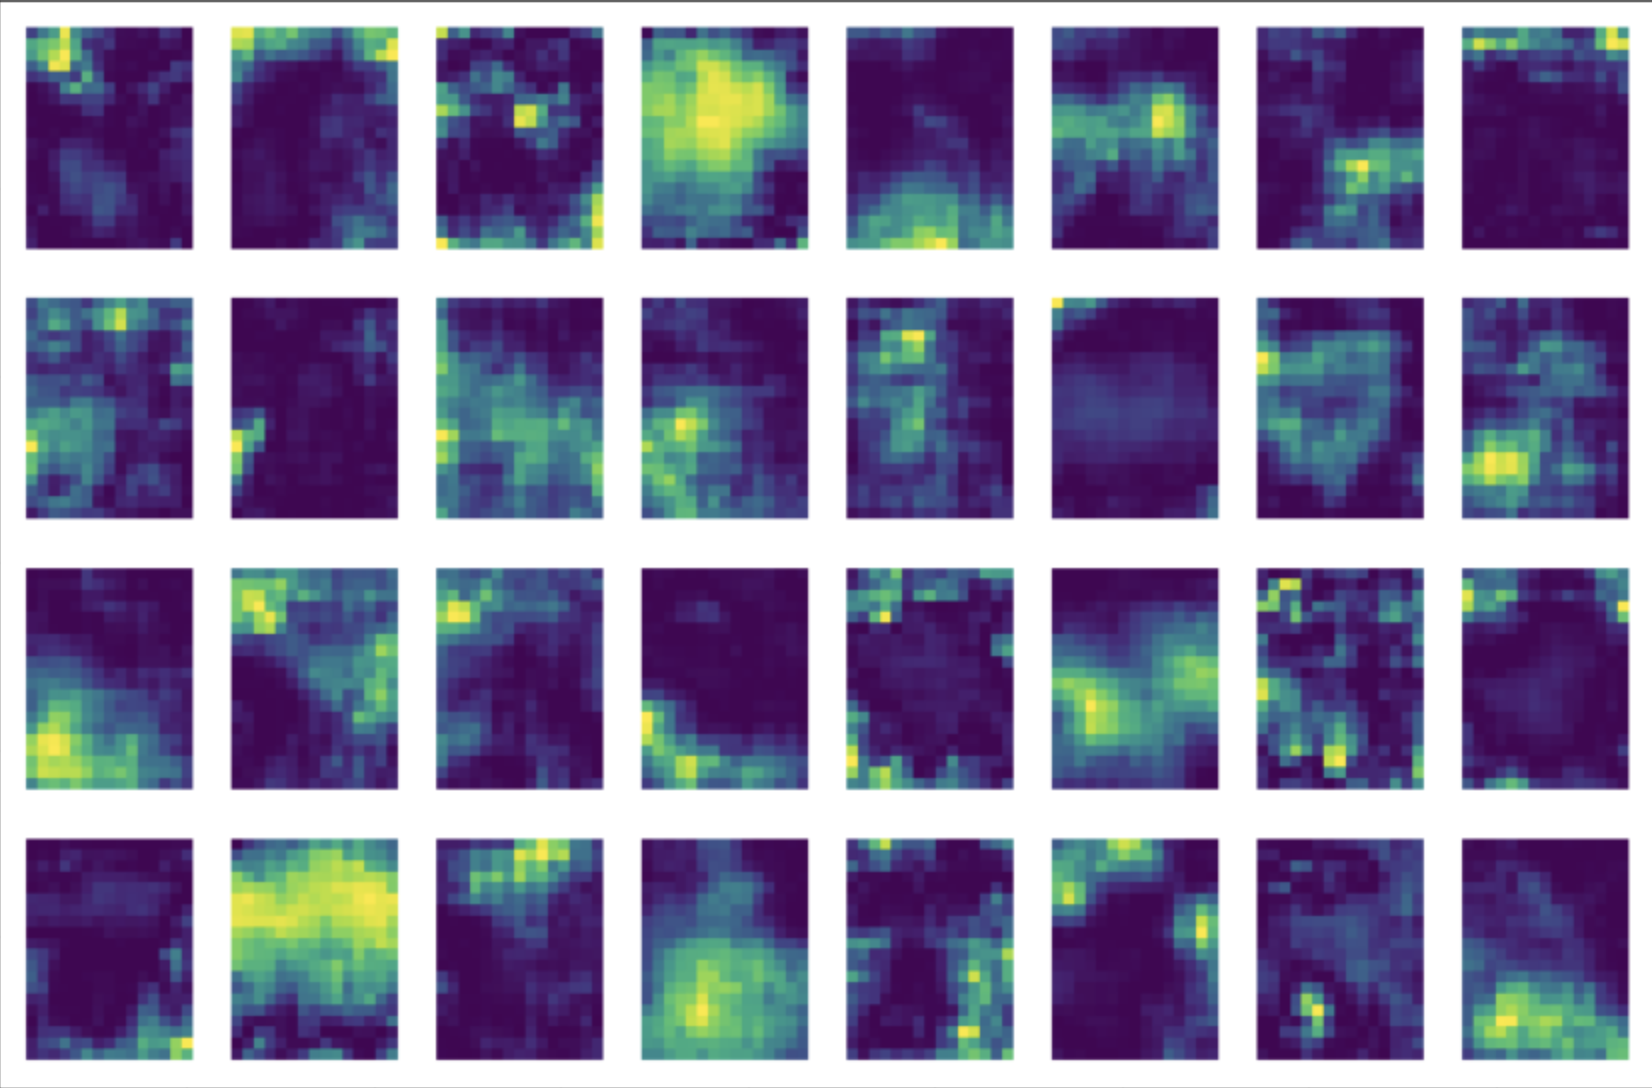
\includegraphics[width=0.7\linewidth]{images/stage9_SPPF_features}
        \caption{Визуализация элементов последнего слоя backbone части модели YOLOv5}
        \label{fig:stage9_SPPF_features}
    \end{figure}

    В качестве признаков для модели регрессии выбирался центральный вектор карты признаков и еще $N - 1$ ближайших к нему векторов, $N = (N_{neig} \cdot 2 + 1)^2$, где $N_{neig}$ - максимальное отклонение от центрального вектора по одной из координат.
    Положение центрального вектора карты признаков определяется формулой $x_c =\left[\left( [\frac{w}{s}]+1\right) \cdot 0,5\right],$ где $w$~--~размер изображения, $s$~--~размер элемента карты признаков.
    Для каждого из $N$ векторов-признаков значение ключевой точки пересчитывалось с учетом расположения данного вектора относительно центра по формуле $x' = \frac{x}{s} - (x_v + 0,5)$, где $x$~--~ключевая точка, $x_v$~--~положение вектора-признака

    Во время применения подхода для нахождения каждой ключевой точки использовались $N$ векторов-признаков, а в качестве предсказания бралось среднее значение всех $N$ прогнозов линейной регрессии на векторах-признаках.
    Преобразование каждого предсказания модели в значение ключевой точки осуществлялось по формуле $x_p = (x'_p + x_c) * s$, где $x'_p$ - предсказание модели.

    Стоит отметить некоторые особенности реализации данного подхода.
    Карта признаков модели YOLOv5 для конкретного изображения могла отличаться при применении модели к набору изображений и к одному изображению в отдельности~--~это обусловлено предобработкой изображений внутри модели с учетом максимального размера изображения в подаваемом наборе.
    В связи с этим перед применением модели YOLOv5 каждое изображение предобрабатывалось: осуществлялось масштабирование и заполнялись края изображения (padding)~--~для получения изображения размера 640×640.
    Для такого изображения матрица имела размерность 20×20.
    Изображения с таким размером модель YOLOv5 дополнительно не предобрабатывала.
    Однако для обучения модели требовалось применить соответствующие преобразования к ключевым точкам - провести масштабирование и сместить на некоторое расстояние от границы изображения.
    Далее к предсказанным моделью ключевым точкам применялось обратное преобразование.

    Поскольку размер вектора из карты признаков намного превышает размер обучающей выборки, состоящей из нескольких примеров, то к признакам модели регрессии применялся метод главных компонент (PCA) для понижения размерности пространства признаков.

    К обучающей части данных также применялись аугментации: изменения цвета, яркости, поворот и кадрирование изображения. Подробнее о проведенных экспериментах изложено в п.~\ref{kpoints_exp}.

	%TODO поменять порядок
    \subsection{Алгоритм улучшения результатов выдачи}

    Предобученные модели могут не выделять или выделять некачественно интересующие пользователя объекты.
    Для решения этой проблемы был реализован алгоритм по улучшению результатов выдачи пайплайна по выделению регионов изображения.

    Была добавлена возможность выбора картинок, которые соответствуют пользовательскому запросу, указанию нерелевантных или загрузки пользовательских изображений, содержащих заданные объекты.
    После пользователь может или оставить предложенные регионы для выбранных изображений, или скорректировать их.
    Далее на полученной разметке выполняется дообучение модели выделения регионов.
    В случае малого количества наблюдений может быть произведена заморозка части весов сети~\cite{wang2020few}.
    Полученную модель можно использовать как самостоятельную для поиска регионов изображений, соответствующим интересующим объектам, так и для повторного запуска на выборке и создания новой модели для поиска по текстовому запросу.

    \subsection{Демонстрация результатов работы предложенного алгоритма детекции объектов}

    %TODO Про демо в ноутбуке и демо сайтик: какие функции, какие классы, какой функционал, как реализовано (либа)

    \subsection{Результаты экспериментов}

    \subsubsection{Поиск ближайших соседей}

    Для оценки качества алгоритмов поиска ближайших соседей был проведен эксперимент.
    В качестве поисковой базы использовались эмбеддинги областей изображений, полученные для валидационной выборки датасета LVIS с помощью регионов модели YOLOv5 и эмбеддингов CLIP, в выборке~852831 наблюдений, размерность эмбеддинга~512.
    Для текстовых запросов использовались эмбеддинги определений классов датасета LVIS, в качестве модели для получения текстовых эмбеддингов выступал CLIP, в выборке~1203 класса.
    В качестве меры близости использовалось косинусное сходство.
    Стоит отметить, что особенность такого датасета~--~относительно низкое значение схожести для наиболее близких векторов.
    Так, значение метрики около~0,3 соответствует хорошей схожести и на реальных запросах редко оказывается значительно выше этого порога.

    Для подсчета качества алгоритмов поиска ближайших соседей использовалась метрика Recall~\cite{aumuller2020ann}, поскольку количество выданных ответов может быть меньше запрошенных.
    В качестве истинных ответов к запросу брались ближайшие к текстовому запросу 30 областей изображений, полученные с помощью полного перебора.
    Количество правильных ответов алгоритма получались как пересечение объектов, выданных алгоритмом (до 30), и истинных ответов.
    Метрика для одного текстового запроса получалась как доля правильных ответов алгоритма.
    Итоговая метрика усреднялась по всем текстовым запросам.

    Для тестирования были выбраны библиотеки Annoy~\cite{annoy}, ScaNN~\cite{avq_2020}, Hnswlib (NMSLIB)~\cite{malkov2018efficient}, а также полный перебор.
    В алгоритме Annoy происходил подбор количества деревьев, которые разделяют пространство признаков.
    В алгоритме ScaNN происходил подбор количества листьев, доли листьев, используемых в итоговом поиске, количество кандидатов, для которых будет произведен точный расчет расстояния до заданного вектора.
    В алгоритме Hnswlib подбиралось количество ребер для каждой вершины, сложность построения графа, способ постобработки результатов.

    Тестирование проводилось на виртуальной машине с~32 vCPU Intel Xeon Processor (Icelake), 64ГиБ оперативной памяти, Ubuntu~20.04.3~LTS, Python~3.8.10.

    На графике~\ref{fig:ann_recall_qps} представлена зависимость метрики Recall от скорости алгоритма (количества запросов в секунду).
    Различное количество запросов для одного алгоритма обусловлено перебором гиперпараметров, влияющих на скорость и точность.
    Красной точкой на графике отмечен полный перебор~--~он имеет идеальную точность (с помощью него осуществлялся выбор правильных ответов), но наиболее медленное время выполнения.
    Можно сделать вывод, что на исследуемом наборе данных алгоритм Annoy работает хуже алгоритмов ScaNN и NMSLib и по скорости, и по точности.
    Наиболее быстрым является алгоритм NMSLib, наиболее точным~--~ScaNN.

    \begin{figure}[H]
        \centering
        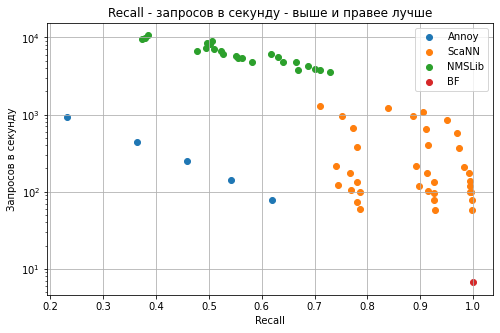
\includegraphics[width=0.7\linewidth]{images/ann_recall_qps}
        \caption{Recall - запросов в секунду - выше и правее лучше}
        \label{fig:ann_recall_qps}
    \end{figure}

    На рис.~\ref{fig:ann_recall_build} представлен анализ времени построения индекса алгоритма и точности.
    Алгоритм ScaNN имеет наименьшее время построения индекса, а Annoy и NMSLib примерно одинаковое, в зависимости от параметров модели.

    \begin{figure}[H]
        \centering
        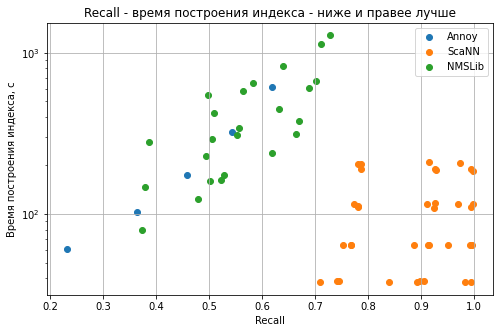
\includegraphics[width=0.7\linewidth]{images/ann_recall_build}
        \caption{Recall - время построения индекса~--~ниже и правее лучше}
        \label{fig:ann_recall_build}
    \end{figure}

    \subsubsection{Анализ подхода к детекции объектов по произвольному запросу} \label{fsod_exp}

	Для оценки качества подхода к детекции объектов был произведен расчет метрики average precision (AP).
	Данная метрика оценивает, насколько хорошо предложенные регионы соответствуют действительным прямоугольным областям, ограничивающих объекты.
	
	$$ AP = \sum_{t} (R_t - R_{t - 1}) P_t $$
	
	Для расчета метрики требуется предварительно вычислить, совпадает ли каждый предложенный регион с истинным.
	Совпадающей считается такая пара, для которой $IoU$ выше заданного порога.
	Кроме того, необходимо определить значение уверенности в конкретном регионе (confidence).
	Далее перебираются все возможные пороги $t$ для уверенности и рассчитываются метрики precision $P_t$ и recall $R_t$.
	$AP$ считается как сумма всех $P_t$, умноженных на приращение $R_t - R_{t - 1}$.
	
	В качестве метрики уверенности использовалось косинусное сходство (distance), а также уверенность модели в конкретном регионе (confidence).
	
	Была проведена оценка следующих комбинаций моделей:
	\begin{enumerate}
		[1)]
		\itemsep0em
		\item ViLD с регионами и эмбеддингами, полученных самой моделью~(ViLD);
		\item регионы модели ViLD, эмбеддинги регионов получены с помощью модели CLIP~(ViLD~+~CLIP);
		\item модель с регионами от YOLOv5 и эмбеддингами от CLIP~(YOLO~+~CLIP).
	\end{enumerate}
	 Для поиска ближайших соседей использовался полный перебор, дополнительно оценено качество модели с использованием библиотеки Annoy~(YOLO~+~CLIP~+~Annoy).
	
	%Для текстовых запросов использовались эмбеддинги для определений классов датасета LVIS, в качестве модели для получения эмбеддингов выступал CLIP, в выборке~1203 наблюдений.
	
	Подробные результаты экспериментов доступны в таблице~\ref{tab:experiments_main} в приложении А.
	На рис.~\ref{fig:average_precision_dataset} представлен анализ метрик для каждой модели в зависимости от количества объектов в запросе.
	Можно заметить, что качество модели ViLD хуже всех других моделей.
	Использование методов приближенного поиска ближайших соседей с неоптимально выбранным алгоритмом может привести к падению метрики.
	Так, значение для модели YOLO~+~CLIP~+~Annoy на $0.02 - 0.04$ ниже, чем для аналогичной модели, но без Annoy.
	На базовых (частых) запросах лидирует модель ViLD~+~CLIP, на редких имеет сопоставимое качество с моделью YOLO~+~CLIP.
	
	\begin{figure}[H]
		\centering
		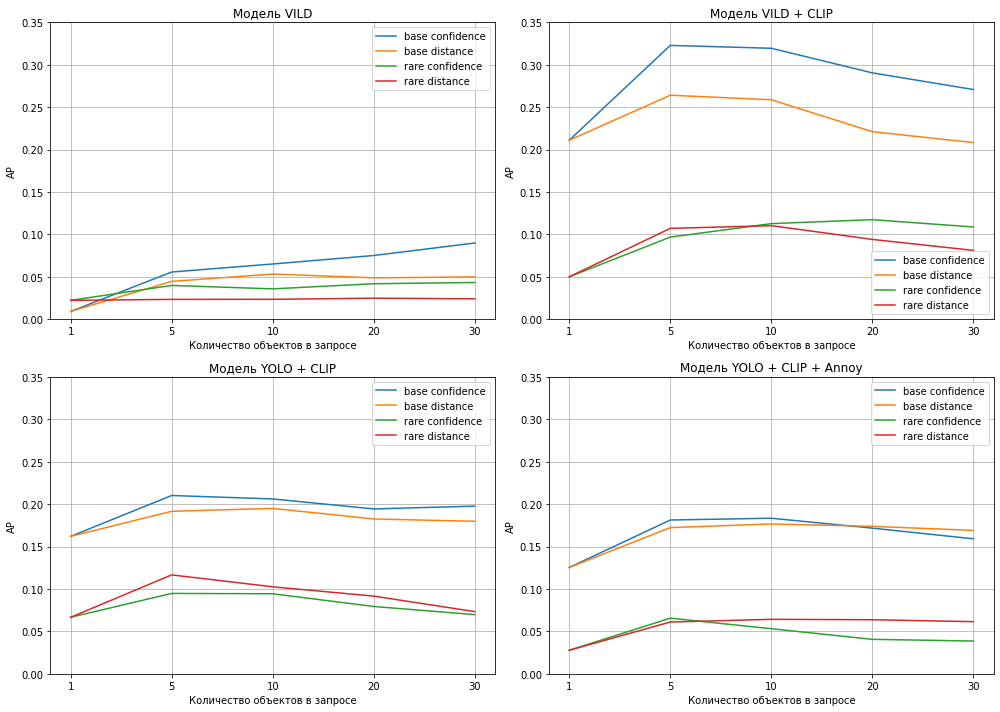
\includegraphics[width=0.999\linewidth]{images/average_precision_dataset}
		\caption{AP в разрезе моделей}
		\label{fig:average_precision_dataset}
	\end{figure}
	
	На рис.~\ref{fig:average_precision_metrics} представлен анализ метрики для моделей в разрезе базовых или редких классов и используемой меры близости или уверенности.
	Из графика следует, что модель YOLO~+~CLIP всегда лучше, чем модель с Annoy.
	На малом количестве соседей (до 5) лидирует модель YOLO~+~CLIP, на большем~--~ViLD~+~CLIP.
	
	\begin{figure}[H]
		\centering
		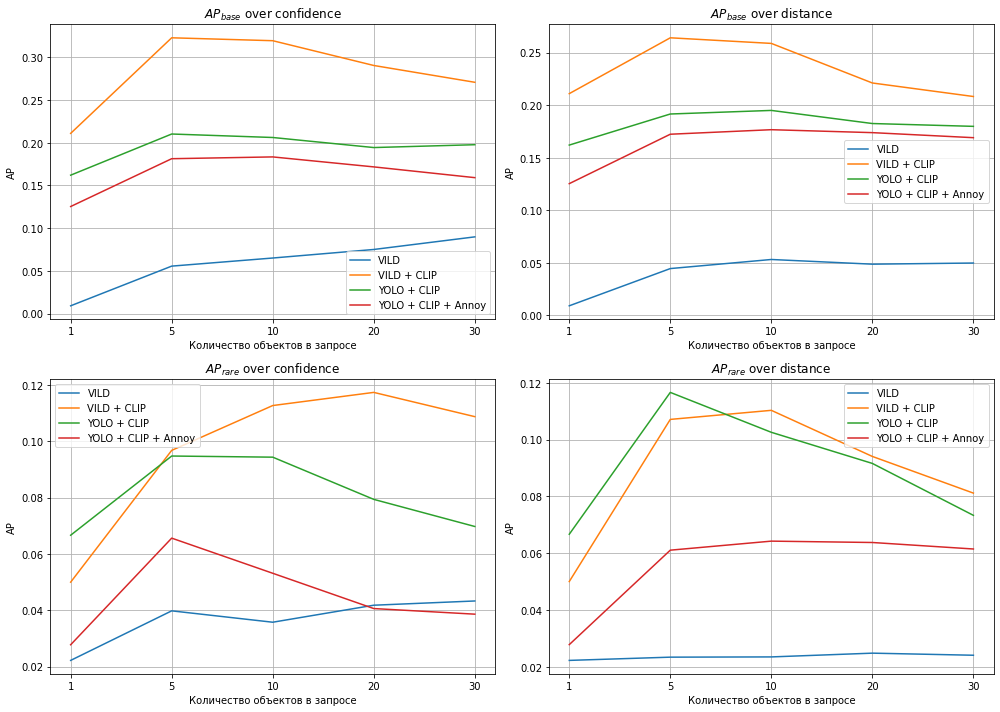
\includegraphics[width=0.999\linewidth]{images/average_precision_metrics}
		\caption{AP в разрезе классов и меры}
		\label{fig:average_precision_metrics}
	\end{figure}

    \subsubsection{Анализ решения задачи регрессии ключевых точек} \label{kpoints_exp}

    Качество предлагаемого подхода к решению задачи регрессии ключевых точек с дообучением по нескольким примерам оценивалось на датасете \cite{cat_dataset}.
    В датасете содержатся более 9000 изображений котов, для каждого изображения содержится разметка из 9 ключевых точек головы животного.
    Пример исследуемых данных представлен на рис.~\ref{fig:example_cat_dataset}.
    Качество применяемых подходов оценивалось с помощью метрик RMSE и $R^2$.
    Замер метрик качества производился для нескольких различных наборов изображений (батчей), в результате оценивались среднее значение и стандартное отклонение метрик.

    \begin{figure}[H]
        \centering
        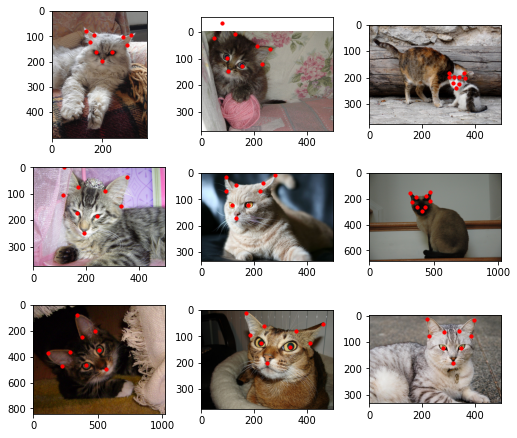
\includegraphics[width=0.6\linewidth]{images/example_cat_dataset}
        \caption{Пример изображений датасета \cite{cat_dataset}}
        \label{fig:example_cat_dataset}
    \end{figure}

    Конфигурация базового эксперимента представлена в таблице~\ref{tab:base_config}.
    \begin{center}
        \begin{table}[H]
            \centering
            \caption{Конфигурация базового эксперимента}
            \label{tab:base_config}
            \bgroup
            \def\arraystretch{1.5}
            \begin{tabular}{| l | r |}
                \hline
                Размер набора изображения         & 32 \\ \hline
                Размер обучающей части            & 16 \\ \hline
                Размер валидационной части            & 8 \\ \hline
                Количество наборов изображений    & 53 \\ \hline
                Максимальное отклонение  $N_{neig}$ & 3  \\
                \hline
            \end{tabular}
            \egroup
        \end{table}
    \end{center}

    При проведении экспериментов для каждого батча осуществлялся подбор оптимального количества компонент PCA по валидационной части. Итоговая модель для проверки на тестовом наборе обучалась на всей обучающей части (совместно с валидационной).
    Пример подбора количества компонент на одном батче для базового эксперимента без аугментаций представлен на рис.~\ref{fig:pca_optim}.

    \begin{figure}[H]
        \centering
        \begin{subfigure}{.5\textwidth}
            \centering
            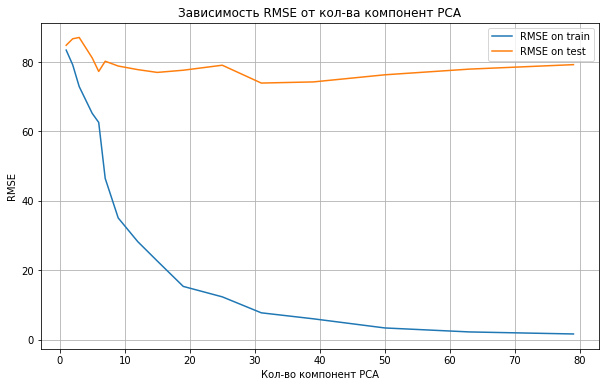
\includegraphics[width=\linewidth]{images/pca_rmse}
            \caption{Зависимость RMSE от количества компонент PCA}
            \label{fig:pca_rmse}
        \end{subfigure}%
        \begin{subfigure}{.5\textwidth}
            \centering
            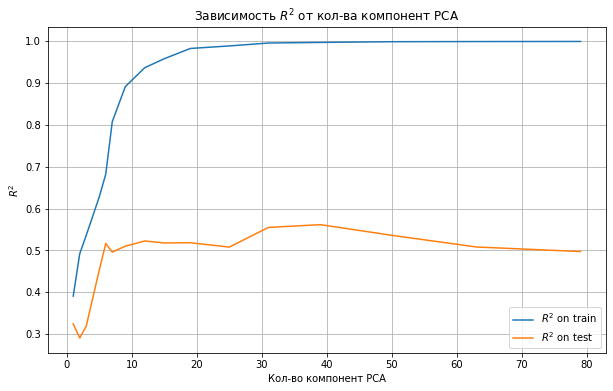
\includegraphics[width=\linewidth]{images/pca_r2}
            \caption{Зависимость $R^2$ от количества компонент PCA}
            \label{fig:pca_r2}
        \end{subfigure}
        \caption{Подбор оптимального количества компонент PCA}
        \label{fig:pca_optim}
    \end{figure}

    Были проведены эксперименты по подбору оптимального количества компонент PCA, оптимальному типу аугментации, применяемому к обучающей части датасета: изменения цвета, яркости, поворота и кадрирования изображения.
    Результаты метрик RMSE и $R^2$ для различных экспериментов представлены в таблицах \ref{tab:experiments_kpoints_rmse} и \ref{tab:experiments_kpoints_r2} соответственно. Для применения случайных аугментаций к изображениям использовалась библиотека Albumentations \cite{albumentations}.

    Также проводился анализ минимального количества изображений в обучающей выборке для решения задачи регрессии ключевых точек, количества аугментаций и оптимального отклонения $N_{neig}$.
    
    В качестве итога можно отметить %TODO итог

    \subsection{Рекомендации по использованию полученных результатов}

    Некоторые распространенные библиотеки для приблизительного поиска ближайших соседей могут работать недостаточно качественно для данной задачи.
    Неправильно выбранный или настроенный алгоритм может значительно повлиять на итоговое качество всего процесса обработки запроса.
    При выборке конкретного варианта стоит обратить внимание на метрики качества используемых алгоритмов, производить подбор гиперпараметров.
    В экспериментах курсовой работы удалось достичь высокого качества ($recall > 0.95$), приемлемого времени построения индекса и скорости работы только для библиотеки ScaNN.

    подход с kpoints - дообучение, аугментации не работает

    какой подход лучше yolo или vild (дообучать модели или нет)

    зашел подход с раскручиванием nms

    Разработанный пайплайн для детекции объектов можно использовать 
        \begin{enumerate}
    	[1)]
    	\itemsep0em
    	\item для отбора наиболее релевантных изображений к запросу из объемного пользовательского датасета и выделения регионов, относящихся к запросу;
    	\item для сбора собственного датасета с выделенными регионами с помощью корректировки регионов, предложенных моделью, и отбором релевантных изображений;
    	\item для получения модели поиска регионов изображений, дообученной  на специфичных запросах.
    \end{enumerate}

    что стоит доработать в демке, что стоит попробовать из моделей, из подходов (+ эксперименты kpoints, что стоит использовать вместо полного перебора, более современные архитектуры (новая статья))
    
    Доработать возможность поиска по картиночному запросу.
    
    В чем отличие предложенного решения от других

    \subsection{Выводы к главе \thesection}
    \begin{enumerate}
        \itemsep0em
        \item Предложен и проанализирован подход к детекции объектов по произвольному текстовому запросу. Исследованы алгоритмы поиска ближайших соседей и модели детекции.
        \item Проведен анализ решения задачи регрессии ключевых точек с дообучением по нескольким примерам.
        \item Приведены рекомендации по использованию полученных результатов работы.
    \end{enumerate}

    \newpage


    \section{Заключение}

    В работе изучена...
    
    Полученные результаты можно применять в ...

    \newpage
    \renewcommand{\refname}{{\normalsize \hfill Список использованных источников \hfill}}
%    \bibliographystyle{unsrt}
    \selectbiblanguage{russian}
    \bibliographystyle{BibTeX-Styles/ugost2008mod}
    \bibliography{main}
    \newpage

    \begin{landscape}

        \begin{flushright}
            \section*{\normalsize \hfill Приложение А \\ \hfill Результаты экспериментов}
        \end{flushright}
        \addcontentsline{toc}{section}{Приложение А}
        \addcontentsline{toc}{subsection}{Результаты экспериментов}

        \begin{table}[H]
            \centering
            \caption{RMSE экспериментов}
            \label{tab:experiments_kpoints_rmse}
            \begin{tabular}{lrrrrr}
                \toprule
                Эксперимент & \makecell{Число \\ компонент PCA } & \makecell{Средняя RMSE \\ на обучении} & \makecell{Стд. отклонение \\ RMSE на обучении} & \makecell{Средняя RMSE \\ на валидации} & \makecell{Стд. отклонение \\ RMSE на валидации} \\
                \midrule
                Базовый эксперимент & 3 & 60,14 & 12,60 & 82,54 & 17,55 \\ \hline
                \makecell{Аугментации \\ цвета и яркости} & 3 & 68,72 & 15,28 & 84,30 & 17,28 \\ \hline
                \makecell{Аугментации цвета,\\ яркости и поворота} & 3 & 69,82 & 15,59 & 84,86 & 17,47 \\ \hline
                \makecell{Аугментации цвета,\\ яркости, поворота \\ и кадрирования} & 3 & 69,69 & 15,46 & 85,30 & 18,29 \\
                \bottomrule
            \end{tabular}
        \end{table}

        \begin{table}[H]
            \centering
            \caption{$R^2$ экспериментов}
            \label{tab:experiments_kpoints_r2}
            \begin{tabular}{lrrrrr}
                \toprule
                Эксперимент & \makecell{Число \\ компонент PCA } & \makecell{Средний $R^2$\\ на обучении} & \makecell{Стд. отклонение \\ $R^2$ на обучении} & \makecell{Средний $R^2$\\ на валидации} & \makecell{Стд. отклонение \\ $R^2$ на валидации} \\
                \midrule
                Базовый эксперимент & 3 & 0,6949 & 0,1222 & 0,4205 & 0,2179 \\ \hline
                \makecell{Аугментации \\ цвета и яркости} & 3 & 0,6063 & 0,1507 & 0,3762 & 0,2663 \\ \hline
                \makecell{Аугментации цвета,\\ яркости и поворота} & 3 & 0,5896 & 0,1571 & 0,3576 & 0,2776 \\ \hline
                \makecell{Аугментации цвета,\\ яркости, поворота \\ и кадрирования} & 3 & 0,5938 & 0,1561 & 0,3521 & 0,2832 \\
                \bottomrule
            \end{tabular}
        \end{table}

        \begin{table}[H]
            \centering
            \caption{метрики AP}
            \label{tab:experiments_main}
            \begin{tabular}{ccc|ccccc|}
%				\toprule
                \cline{4-8}
                & & & \multicolumn{5}{c|}{Количество соседей} \\ \hline
                Модель              & Сегмент & Метрика    & 1               & 5               & 10              & 20              & 30              \\
                \midrule
                VILD                & base    & confidence & 0,0091          & 0,0556          & 0,0651          & 0,0751          & 0,0898          \\
                VILD                & base    & distance   & 0,0091          & 0,0445          & 0,0532          & 0,0487          & 0,0498          \\
                VILD                & rare    & confidence & 0,0222          & 0,0398          & 0,0357          & 0,0418          & 0,0433          \\
                VILD                & rare    & distance   & 0,0222          & 0,0233          & 0,0234          & 0,0247          & 0,0240          \\ \hline
                VILD + CLIP         & base    & confidence & \textbf{0,2110} & \textbf{0,3228} & \textbf{0,3194} & \textbf{0,2904} & \textbf{0,2708} \\
                VILD + CLIP         & base    & distance   & \textbf{0,2110} & 0,2641          & 0,2587          & 0,2211          & 0,2082          \\
                VILD + CLIP         & rare    & confidence & 0,0500          & 0,0967          & \textbf{0,1127} & \textbf{0,1173} & \textbf{0,1087} \\
                VILD + CLIP         & rare    & distance   & 0,0500          & 0,1071          & 0,1103          & 0,0940          & 0,0811          \\ \hline
                YOLO + CLIP         & base    & confidence & 0,1620          & 0,2102          & 0,2061          & 0,1944          & 0,1977          \\
                YOLO + CLIP         & base    & distance   & 0,1620          & 0,1916          & 0,1950          & 0,1825          & 0,1798          \\
                YOLO + CLIP         & rare    & confidence & \textbf{0,0666} & 0,0947          & 0,0943          & 0,0793          & 0,0697          \\
                YOLO + CLIP         & rare    & distance   & \textbf{0,0666} & \textbf{0,1166} & 0,1025          & 0,0916          & 0,0733          \\ \hline
                YOLO + CLIP + Annoy & base    & confidence & 0,1253          & 0,1813          & 0,1834          & 0,1717          & 0,1591          \\
                YOLO + CLIP + Annoy & base    & distance   & 0,1253          & 0,1723          & 0,1767          & 0,1739          & 0,1691          \\
                YOLO + CLIP + Annoy & rare    & confidence & 0,0277          & 0,0656          & 0,0531          & 0,0406          & 0,0386          \\
                YOLO + CLIP + Annoy & rare    & distance   & 0,0277          & 0,0610          & 0,0642          & 0,0637          & 0,0614          \\
                \bottomrule
            \end{tabular}
        \end{table}
    \end{landscape}
\end{document}